\subsection{Go Concurrency}
\label{sec:goConcurrency}
%
%\stcmtside{Go concurrency introduction}
Go introduces a new concurrency model, mixing shared-memory and message-passing concepts with an ad-hoc scheduler:
\begin{itemize}
    \item \textbf{Goroutines} are functions that execute concurrently on logical processors having their own stack.
    \item \textbf{Channels} are typed conduits through which goroutines communicate.  Channels are unbuffered by default, providing synchronous (rendezvous) messaging between goroutines.
    \item \textbf{Synchronization} features such as \textit{(RW)mutex}, \textit{waitGroup}, \textit{conditional variables}, \textit{select}, and \textit{context} are included in the language to provide more and flexible synchronization, data access serialization, memory protection, and error handling.
    \item \textbf{Scheduler} maintains goroutines in FIFO queues and binds them on OS threads to execute on processing cores.
\end{itemize}

\ignore{Due to the unpredictable interaction between components and inherent non-determinism introduced by the scheduler, concurrent programming and debugging has traditionally been challenging.
%
}

%\begin{listing}[]
\begin{minipage}{.5\textwidth}
\begin{minted}
[
fontsize=\scriptsize,
linenos=true,
escapeinside=||,
breaklines
]
{go}
package main
import "sync"

type Container struct{ |\label{bugListing:containerType_start}|
  sync.Mutex
  stop  chan struct{}
} |\label{bugListing:containerType_end}|

func main() {
  container := &Container{ |\label{bugListing:container_create_start}|
       stop:make(chan struct{})} |\label{bugListing:container_create_end}|
  go Monitor(container) |\label{bugListing:main_go_monitor}|
  go StatusChange(container) |\label{bugListing:main_go_statChange}|
}
\end{minted}
\end{minipage}
\begin{minipage}{.35\textwidth}
\begin{minted}
[
fontsize=\scriptsize,
linenos=true,
escapeinside=||,
breaklines
]
{go}
|\setcounter{FancyVerbLine}{15}|func Monitor(cnt *Container){
  for{
    select{
    case <- cnt.stop:  |\label{bugListing:Monitor_case_recv}|
      return |\label{bugListing:Monitor_case_recv_ret}|
    default: |\label{bugListing:Monitor_case_def}|
      cnt.Lock()  |\label{bugListing:Monitor_case_def_lock}|
      cnt.Unlock() |\label{bugListing:Monitor_case_def_unlock}|
}}}
func StatusChange(cnt *Container){
  cnt.Lock() |\label{bugListing:statChange_lock}|
  cnt.stop <- struct{}{} |\label{bugListing:statChange_send}|
  cnt.Unlock() |\label{bugListing:statChange_defer_unlock}|
}
\end{minted}
\end{minipage}
\begin{minipage}{.29\textwidth}
  \centering
  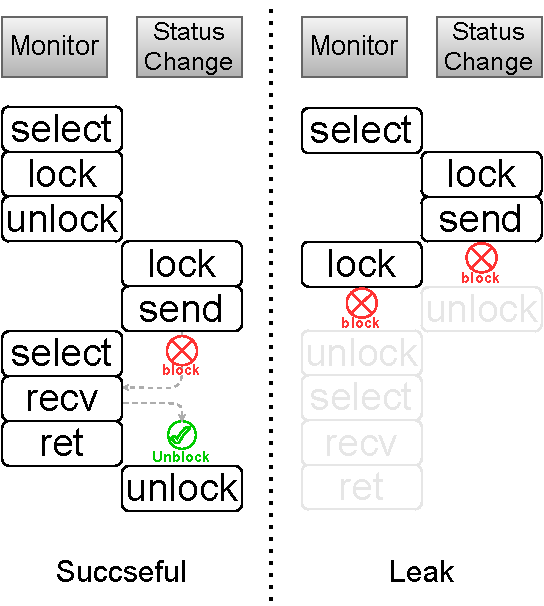
\includegraphics[width=.99\linewidth]{figs/execViz_moby.pdf}
\end{minipage}
\caption{Simplified version of bug \texttt{moby28462}}
\label{listing:moby28462}
\end{listing}

\begin{listing*}[]
\begin{minipage}{.35\textwidth}
\begin{minted}
[
fontsize=\footnotesize,
linenos=true,
escapeinside=||,
breaklines
]
{go}
package main
import "sync"

type Container struct{ |\label{bugListing:containerType_start}|
  sync.Mutex
  stop  chan struct{}
} |\label{bugListing:containerType_end}|

func main() {
  container := &Container{ |\label{bugListing:container_create_start}|
       stop:make(chan struct{})} |\label{bugListing:container_create_end}|
  go Monitor(container) |\label{bugListing:main_go_monitor}|
  go StatusChange(container) |\label{bugListing:main_go_statChange}|
}
\end{minted}
\end{minipage}
\begin{minipage}{.35\textwidth}
\begin{minted}
[
fontsize=\scriptsize,
linenos=true,
escapeinside=||,
breaklines
]
{go}
|\setcounter{FancyVerbLine}{15}|func Monitor(cnt *Container){
  for{
    select{|\label{bugListing:Monitor_select}|
    case <- cnt.stop:  |\label{bugListing:Monitor_case_recv}|
      return |\label{bugListing:Monitor_case_recv_ret}|
    default: |\label{bugListing:Monitor_case_def}|
      cnt.Lock()  |\label{bugListing:Monitor_case_def_lock}|
      cnt.Unlock() |\label{bugListing:Monitor_case_def_unlock}|
}}}
func StatusChange(cnt *Container){
  cnt.Lock() |\label{bugListing:statChange_lock}|
  defer cnt.Unlock() |\label{bugListing:statChange_defer_unlock}|
  cnt.stop <- struct{}{} |\label{bugListing:statChange_send}|
}
\end{minted}
\end{minipage}
\begin{minipage}{.25\textwidth}
  \centering
  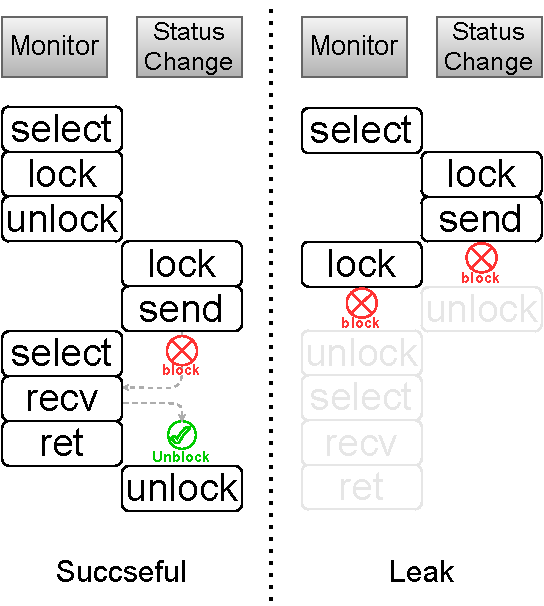
\includegraphics[width=.99\linewidth]{figs/execViz_moby.pdf}
\end{minipage}
\caption{Simplified version of bug \texttt{moby28462}}
\label{listing:moby28462.minipage}
\end{listing*}

%\begin{listing}[]
\begin{minipage}{.45\columnwidth}
\begin{minted}
[
fontsize=\footnotesize,
linenos=true,
escapeinside=||,
xleftmargin=2em,
breaklines
]
{go}
package main
import "sync"

type Cont struct{|\label{bugListing:containerType_start}|
  sync.Mutex
  stop  chan struct{}
}|\label{bugListing:containerType_end}|

func main() {
  cnt := &Cont{|\label{bugListing:container_create_start}|
       stop:make(chan struct{})}|\label{bugListing:container_create_end}|
  go Monitor(cnt)|\label{bugListing:main_go_monitor}|
  go StatusChange(cnt)|\label{bugListing:main_go_statChange}|
}
\end{minted}
\end{minipage}\hfill
\begin{minipage}{.45\columnwidth}
\begin{minted}
[
fontsize=\footnotesize,
linenos=true,
escapeinside=||,
breaklines
]
{go}
|\setcounter{FancyVerbLine}{15}|func Monitor(cnt *Cont){
  for{
    select{
    case <- cnt.stop:  |\label{bugListing:Monitor_case_recv}|
      return |\label{bugListing:Monitor_case_recv_ret}|
    default: |\label{bugListing:Monitor_case_def}|
      cnt.Lock()  |\label{bugListing:Monitor_case_def_lock}|
      cnt.Unlock() |\label{bugListing:Monitor_case_def_unlock}|
}}}
func StatusChange(cnt *Cont){
  cnt.Lock() |\label{bugListing:statChange_lock}|
  defer cnt.Unlock() |\label{bugListing:statChange_defer_unlock}|
  cnt.stop <- struct{}{} |\label{bugListing:statChange_send}|
}
\end{minted}
\end{minipage}
\caption{Simplified version of bug \texttt{moby28462}}
\label{listing:moby28462}
\end{listing}



%\stcmtside{Explaining the example to motivate}
Listing \ref{listing:moby28462.minipage} shows a simplified version of a reported bug in Docker \cite{moby-28462-commit}.
%
An instance of the \texttt{Container} type (lines \ref{bugListing:containerType_start}-\ref{bugListing:containerType_end}) is created in the \texttt{main} function (lines \ref{bugListing:container_create_start}-\ref{bugListing:container_create_end}).
%
In line \ref{bugListing:main_go_monitor}, a goroutine is spawned to execute function \texttt{Monitor} that continuously checks the container status and returns once it receives from the container's channel (lines \ref{bugListing:Monitor_case_recv}-\ref{bugListing:Monitor_case_recv_ret}).
%
The default case of the \texttt{select} statement (line \ref{bugListing:Monitor_case_def}) allows \texttt{Monitor} to continue monitoring without getting blocked on the channel receive (line \ref{bugListing:Monitor_case_recv}).
%
Concurrent to the \texttt{main} and \texttt{Monitor} goroutines, another goroutine is created in line  \ref{bugListing:main_go_statChange} to execute function \texttt{StatusChange} which changes the status of the container by sending to the container's channel.
%
The container's lock is released after the send action completes and function returns (\texttt{defer} statement in line \ref{bugListing:statChange_defer_unlock}).
%


Native execution of this program terminates successfully without issuing any error or warning.
%
Based on the Go specification and memory model, there is no constraint on the goroutines spawned from the \texttt{main} function to join back before the \texttt{main} goroutine\footnote{In the remainder of the paper, we use \textit{main function} and \textit{main goroutine} interchangeably.} terminates.
%
A deadlock detector within the runtime periodically checks that the scheduler queues of all \textit{runnable} goroutines never become empty until the \texttt{main} goroutine terminates.
%
In other words, the runtime throws a deadlock exception when the \texttt{main} goroutine is blocked, and no other goroutine is in the queue to execute (\ie \textit{global deadlock}).
%
Since there is no blocking instruction in the \texttt{main} goroutine in listing \ref{listing:moby28462.minipage}, the program terminates successfully regardless of other goroutines' statuses.
%
However, this program suffers from a common bug in concurrent Go where one or more goroutines \textit{leak} (\ie \textit{partial deadlock}) from the execution (\ie never reach their end states).

%\stcmtside{Explain the deadlock (leak) situation that might get overlooked}
Due to the non-determinism introduced by the runtime scheduler and application-level random features like \texttt{select}, many interleavings are feasible for concurrent execution of simple programs such as listing \ref{listing:moby28462.minipage}.
%
The right side of the listing displays a successful and a \textit{leaky} interleaving of the program.
%
In the leaky scenario, first, the \texttt{Monitor} goroutine executes the \texttt{select} statement and, based on the available cases, picks the default case to execute.
%
Right before the execution of mutex lock (line \ref{bugListing:Monitor_case_def_lock}), the scheduler context-switches and the \texttt{StatusChange} goroutine starts its execution through which it holds the lock and blocks on sending to the channel (line \ref{bugListing:statChange_send}) since there is no receiver on that channel.
%
Upon blocking on send, the scheduler transfers back the control to the \texttt{Monitor} goroutine that tends to acquire the mutex, but because the mutex is already held by \texttt{StatusChange}, the \texttt{Monitor} goroutine also blocks.
%
The circular wait between the container mutex and channel prevents both spawned goroutines from reaching their end states and leaves the program in an unnoticed deadlock situation.
%
\stcmtside{The thirst for novel and scalable debuggers}
Widely used deadlock detectors such as Goodlock \cite{havelund-goodlock-spin00} are not applicable in Go since causes of Go deadlocks are resources (\eg locking a locked mutex) or communication (\eg sending on a full channel), or a combination of them (\eg leaky interleaving of listing \ref{listing:moby28462.minipage}).
%
In addition, due to the light-weight nature of goroutines, it is not uncommon to spawn thousands of goroutines in production software systems.
%
Hence,  novel and scalable techniques are needed to enable realistic modeling of program behavior during execution.
%


\subsection{Concurrency Bugs in Go}
\label{sec:goBugs}
Based on a proposed bug taxonomy for Go \cite{tu-concurrentBugs-asplos19}, bugs are categorized separately based on their \textit{causes} (shared-memory vs. message-passing) and \textit{symptoms} (blocking vs. non-blocking).
%
Blocking bugs historically refer to situations where one or more processing units (\eg goroutines) are blocked, waiting for an external signal to resume (\eg deadlock situation in listing \ref{listing:moby28462_minipage}).
%
The observed causes of such blocking flaw in the context of Go are as follows:

\begin{itemize}
  \item \textit{Resource deadlocks}: Go inherits resource deadlocks from multithreaded languages like Java and C/Pthreads where threads (goroutine in Go) are trapped in a circular wait for the resource (\eg mutex, conditional variable, semaphore, etc.) that is holded by other threads (goroutines).
  \item \textit{Communication deadlocks}: Synchronized (unbuffered) channels transmit values from one goroutine to another in a rendezvous fashion. The sender (or receiver) blocks until the receiver (or sender) is ready to receive (send). Misuse of channel operations might result in one or more goroutines waiting for a sender/receiver to unblock them forever.
  \item \textit{Mixed deadlocks}: There are situations when goroutine $A$ is holding a resource (\eg locked a mutex) while blocking on a channel receive and goroutine $B$ is the sender (unblocker) for $A$ but it requires to hold the mutex lock before sending to $A$.
\end{itemize}
\stcmtside{about race}
Go inherited traditional non-blocking bugs such as data races and atomicity violations from older concurrent languages while introducing new bug idioms due to its new concepts such as anonymous functions \cite{tu-concurrentBugs-asplos19}.
%
\noindent{\bf Sources of non-determinism:\/}
In addition to non-deterministic nature of concurrent languages, Go introduces some level of non-determinism in application level.
%
The \texttt{select} statement gives the flexibility to the program design to randomly select \stcmt{I will complete this about select}

\subsection{Current Correctness Tooling}

Decades of research effort have been dedicated to the logical and performance correctness of concurrent and parallel programs.
%
For CSP-based concurrent languages like Go, static (source-level) analysis methods \cite{ng-dl-cc16,lange-fence-popl17,lange-staticType-icse18} tend to assure bug freedom and verify safety properties through abstractions like session types and choreography synthesis.
%
Ng and Yoshida \cite{ng-dl-cc16} first proposed a static tool to detect global deadlock in Go programs using choreography synthesis.
%
Later, Stadtmuller et al. \cite{stadtmuller-minigo-aplas16} proposed a static trace-based global detection approach based on forkable regular expressions.
%
Lange et al. proposed more static verification frameworks for checking channel safety, and liveness \cite{lange-fence-popl17}, and behavioral model checking \cite{lange-staticType-icse18}.
%
Both methods approximate Go programs with session types and behavioral contracts extracted from their SSA intermediate representation.
%
The mentioned work has limitations for handling dynamic (e.g., in-loop) goroutine or channel creation.
%
They also do not scale and are impractical in real-world programs due to the state explosion problem and lack of proper front-end interface \cite{yuan-gobench-cgo21}.
%
Besides, similar to other static analysis methods, they often suffer from false positives due to conservative constraints.

%
Dynamic (runtime-level) analysis approaches \cite{sulzmann-twophase-2018,dilley-gomela-corr2020} rely on code instrumentation and program rewrites to obtain and analyze an \textit{execution model}.
%
Zhao et al. \cite{zhao-occam97} introduced a runtime monitoring approach for deadlock detection for Occam programs based on wait-for graphs and some heuristics. Occam is a concurrent language based on CSP semantics, and similar to Go, it uses channels to establish communication between processes.
%
Sulzmann and Stadtmuller proposed a dynamic verification approach for synchronous (unbuffered) channels \cite{sulzmann-corr17}, and a vector-clock-based approach for asynchronous channels \cite{sulzmann-twophase-2018}.
%
Although they may support a larger subset of the Go language, they only focus on channels as the root cause of deadlocks and evaluated only on relatively small examples.
%
Also, they usually do not scale for real-world Go applications with thousands of goroutines and LOC \cite{dilley-empirical-saner19}.
%

Standard Go comes with a few dynamic analysis tools. For example, the \textit{race detector} \cite{go-race-blog} which is basically a wrapper around ThreadSanitizer \cite{konstantin-tsan-wbia09}, tracks memory accesses and detect races that happened during execution.
%
A few other facilities for code coverage measurement, profiling, and tracing \cite{go-package-trace} are provided to deliver insight into the testing quality and performance behavior.
%
The built-in race detector \cite{go-race-blog}, despite its limitations (\eg supporting up to 8192 goroutines), has proved to be effective in dynamically detecting data races in most cases quickly.
%
In this work, our focus is on blocking bugs as they have received little attention.

\stcmtside{motivates dynamic tracing}
It is crucial for debuggers and software analysis tools to construct their abstract models as close as possible to the actual program execution context.
%
For multi-threaded Java, effective dynamic methods like ConTest \cite{contest-jgi01}, Goodlock \cite{havelund-goodlock-spin00} and CalFuzzer \cite{joshi-calfuzzer} maintain a model built from \textit{synchronization constructs} of the program, as the main ingredient of dynamic concurrency model.
%
Our investigations state that such comprehensive dynamic data collection mechanisms to abstract reliable concurrency models for Go applications do not exist.
%
Profilers \cite{go-profile-blog} give up some accuracy by approximating the dynamic behavior through aggregated samples from counters,
%
while distributed (decentralized) tracing systems \cite{dapper} gather logs and information (\eg HTTP request latency) through source instrumentation and an underlying network.
%
We explain the enhancement that we made to the original tracer package of Go to obtain accurate reflection of dynamic concurrent behavior of Go applications in section \ref{sec:design}
%


\subsection{Accelerating bug exposure}

\stcmt{
- background on testing, schedule-space exploration, accelrating bug Exposure
}


\stcmt{related work for testing and schedule-exploration}
Systematic testing combines ideas from static and dynamic approaches to reduce the state space and reflect realistic behavior.
%
Assuming the scheduler causes concurrency bugs (and not the program input), they may not manifest during conventional testing and difficult to reproduce, both due to non-deterministic decisions that the scheduler makes.
%
Stress testing the scheduler to examine possible interleaving is useful to expose hidden bugs, but they are exponentially expensive relative to the number of concurrent units.
%
Researchers have applied different methods \cite{thomson-concurrencyTesting-ppopp14} to reduce the interleaving space to explore effectively and efficiently.
%
Delay-bounded \cite{emmi-delayBounded-popl11,burckhardt-depthBug-asplos10} and preemption-bounded \cite{madanlal-preemptionBound-pldi07} techniques systematically ``fuzz'' the scheduler to equally and fairly cover feasible interleaving.
%
Other tools like Maple \cite{yu-maple-oopsla12}, CalFuzzer \cite{joshi-calfuzzer},  and ConTest \cite{contest-jgi01,edelstein2003contest} \textit{actively} control the scheduler to maximise a pre-defined concurrency coverage criterion \cite{hong-syncTesting-issta12} or the probability of bug exposure \cite{burckhardt-depthBug-asplos10}.

Adopting ideas from existing concurrency testing tools, we systematically navigate the scheduler towards executing likely-erroneous interleaving.
%
We first identify the usage of concurrency primitives (\textit{critical points}) in the program using a tracing mechanism.
%
We automatically inject random delays around the critical points to increase the probability of bug exposure (more in section \ref{sec:design}).

\stcmt{maybe one paragraph about coverage}
\stcmt{intro to coverage}
\begin{itemize}
  \item We also have defined a coverage metric/model/criterion To measure the quality of tests that GOAT is able to perform.
  %
  \item Our experiments show that GOAT is effecive in detecting 100\% of blocking bugs in GoKer bench.
  \item Our experiments also show that the coverage metrics that we designed have linear correlation with the rate of bug exposure (i.e., number of testing runs that it takes for the buggy interleaving to occur) for rare bugs.
  \item While these ideas have been developed and proved to be effective in other contexts \cite{burckhardt-depthBug-asplos10,emmi-delayBounded-popl11,madanlal-preemptionBound-pldi07}, our contribution is to show these ideas in the context of a modern language with growing industry-side adoption.
\end{itemize}
